\subsubsection{UC5 - Generazione \glossario{prompt}}\label{UC5}

\begin{figure}[H]
  \centering
  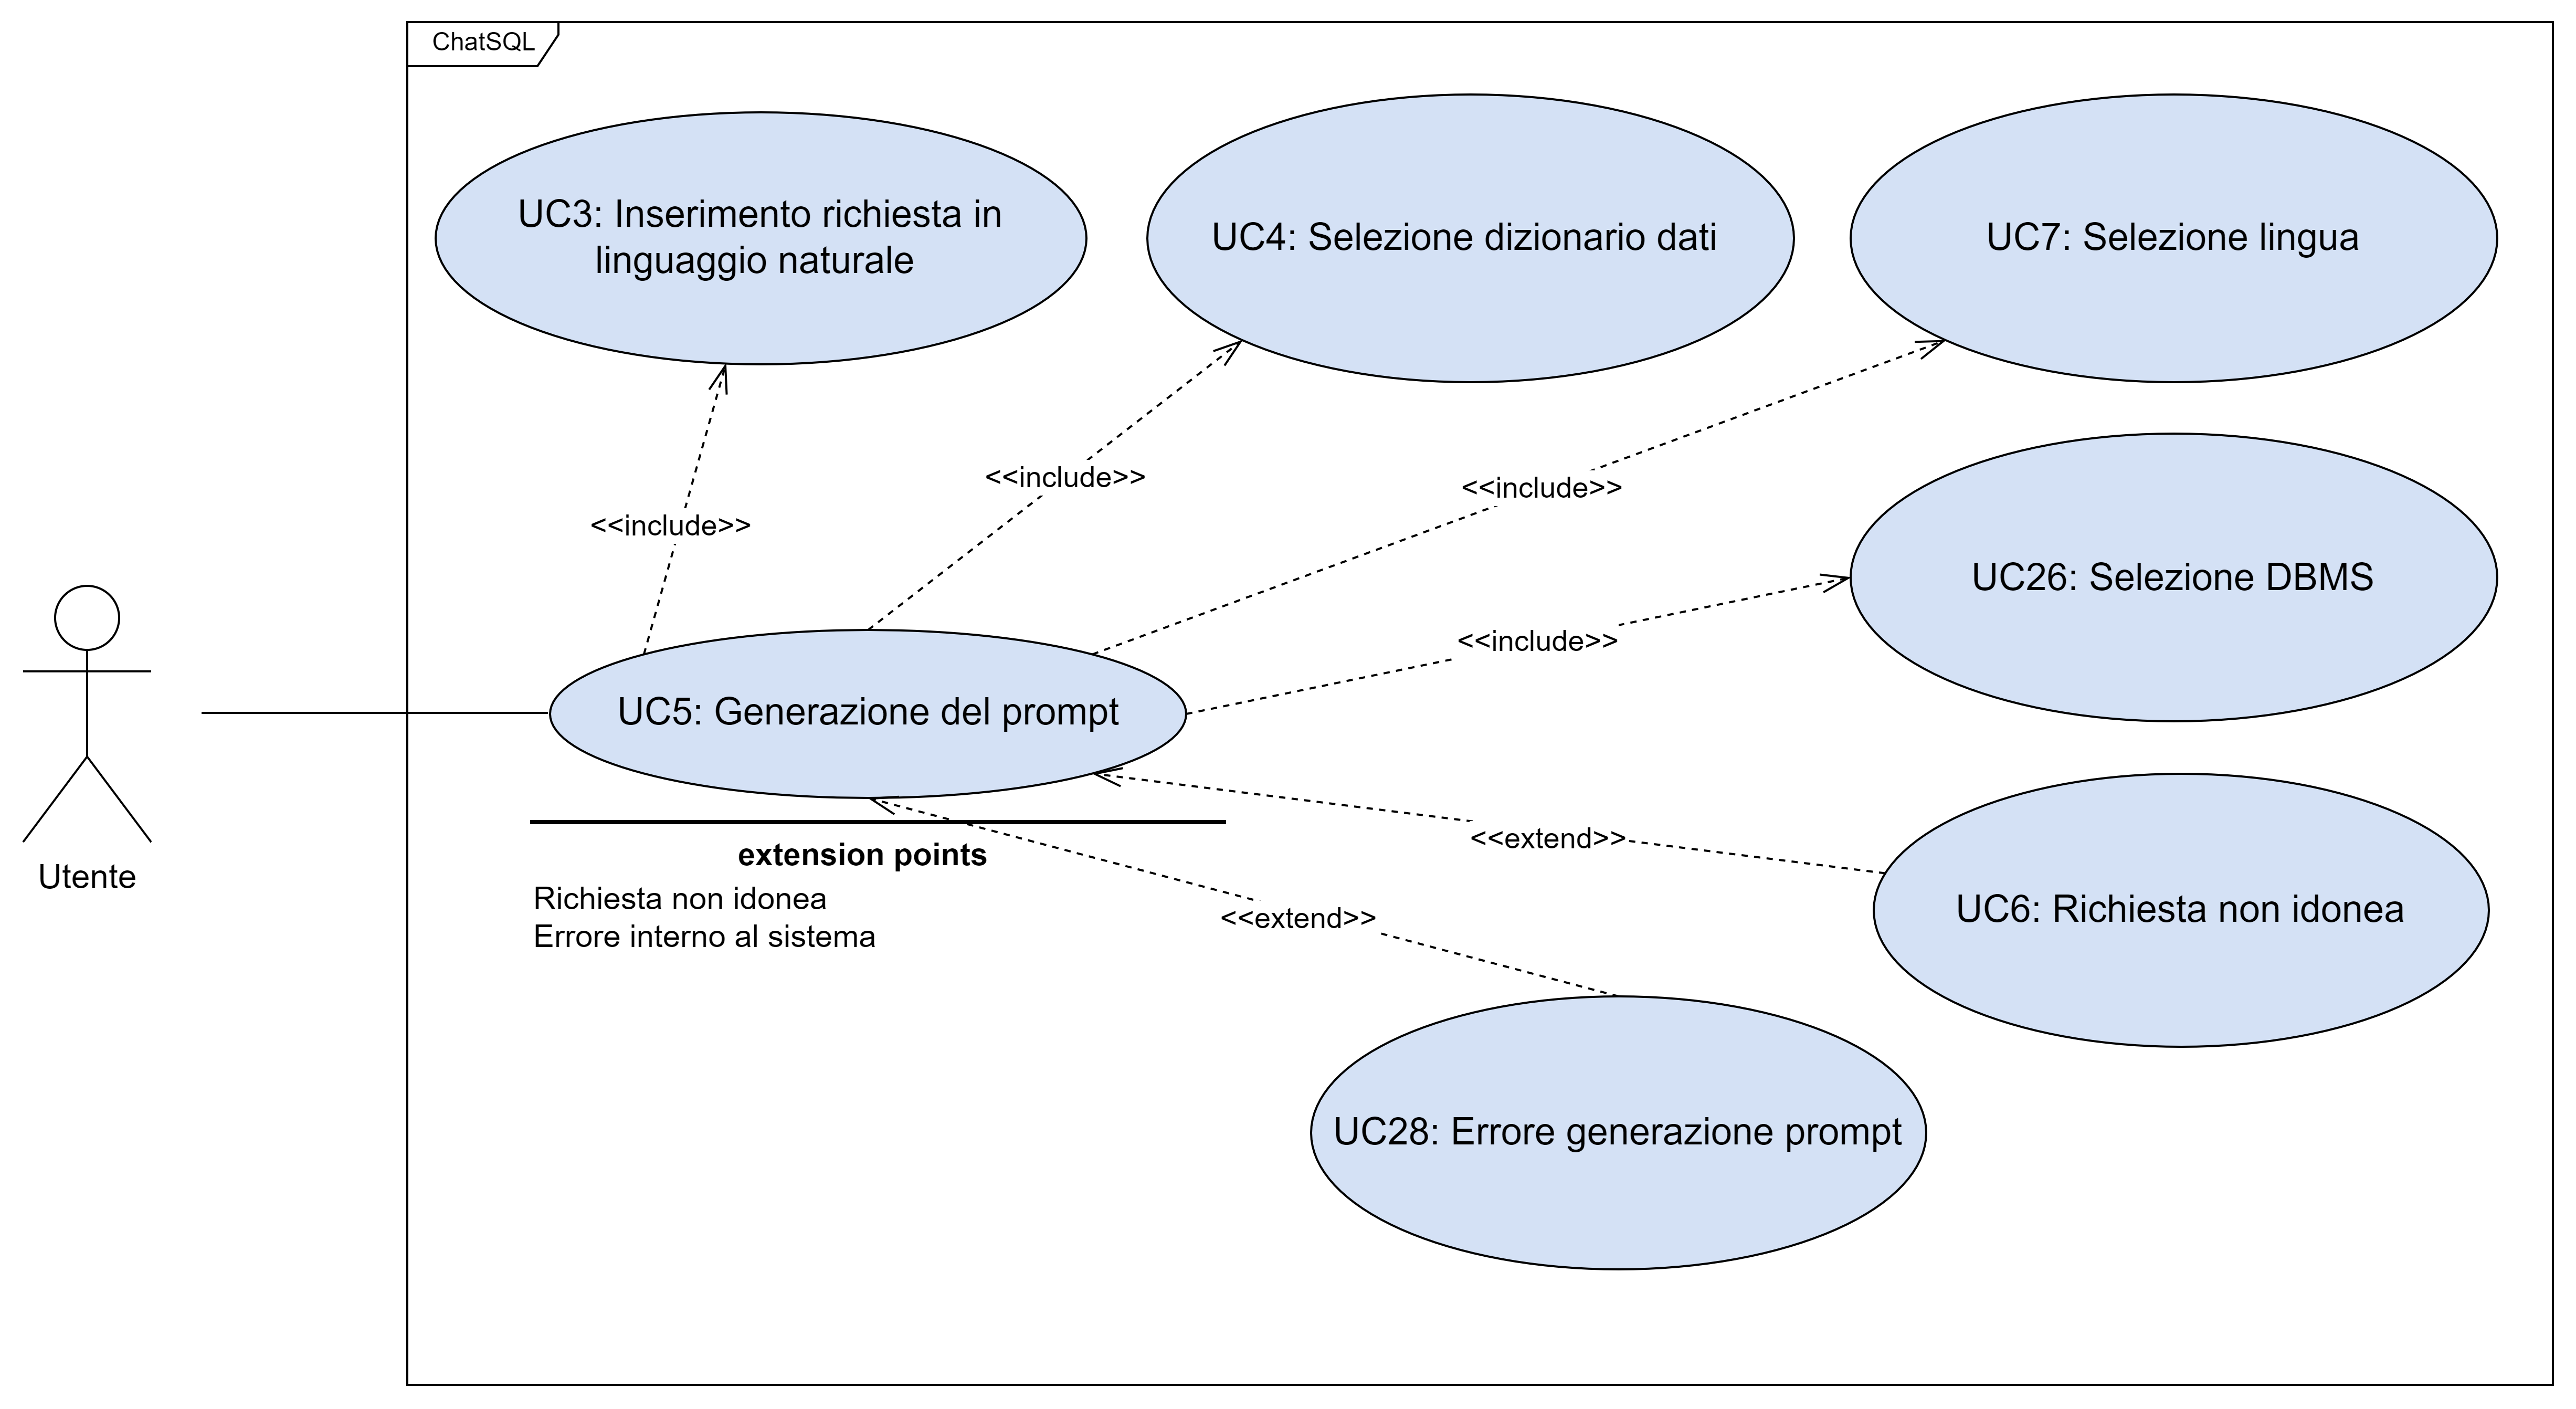
\includegraphics[width=0.90\textwidth]{assets/uc5.png}
  \caption{UC5}
\end{figure}

\paragraph*{Descrizione}
L’Utente desidera ottenere un \glossario{prompt} al fine di utilizzarlo poi con LLM esterni per generare \glossario{\glossario{query}} SQL fornendo parti ristrette di \glossario{dizionario dati}.

\paragraph*{Attori principali}
Utente

\paragraph*{Precondizioni}
\begin{itemize}
  \item L'applicazione è stata avviata con successo;
  \item È presente almeno un \glossario{dizionario dati} nel sistema.
  \item L'Utente ha selezionato un \glossario{dizionario dati} (\hyperref[UC4]{UC4});
  \item L'Utente ha inserito una richiesta in linguaggio naturale (\hyperref[UC3]{UC3}).
\end{itemize}

\paragraph*{Postcondizioni}
\begin{itemize}
  \item Il sistema genera un \glossario{prompt} in base alla richiesta ricevuta e al \glossario{dizionario dati} scelto. Attraverso dei metadati restituisce un \glossario{prompt} con il quale stabilisce quali parti di \glossario{dizionario dati} sono maggiormente necessarie ed efficienti per scrivere la richiesta ricevuta in linguaggio naturale;
  \item L’Utente riceve il \glossario{prompt} generato;
\end{itemize}

\paragraph*{Scenario principale}
\begin{enumerate}
  \item L’Utente desidera ottenere il \glossario{prompt} che permette di generare la \glossario{query} SQL;
  \item L'Utente visualizza la lista dei \glossario{dizionari dati} disponibili (\hyperref[UC10]{UC10});
  \item L'Utente decide di visualizzare un \glossario{dizionario dati} dalla lista (\hyperref[UC9]{UC9});
  \item L’Utente seleziona un \glossario{dizionario dati} sul quale baserà l’interrogazione (\hyperref[UC4]{UC4});
  \item L’Utente inserisce una interrogazione in linguaggio naturale nel box testuale apposito (\hyperref[UC3]{UC3});
  \item Inizia il processo di generazione del \glossario{prompt} e di raccolta di metadati.
\end{enumerate}

\paragraph*{Scenario alternativo}
\begin{enumerate}
  \item Errore nella generazione del \glossario{prompt} (\hyperref[UC6]{UC6}).
  \item Viene visualizzato un messaggio con i dettagli dell'errore.
\end{enumerate}

\paragraph*{Inclusioni}
\begin{itemize}
  \item Inserimento richiesta in linguaggio naturale (\hyperref[UC3]{UC3});
  \item Selezione \glossario{dizionario dati} (\hyperref[UC4]{UC4}).
\end{itemize}

\paragraph*{Estensioni}
\begin{itemize}
  % Inserito anche selezione dizionario dati. Da capire se dopo il prompt si possa interagire nuovamente con la lista
  \item Selezione e copia del \glossario{prompt} risultato (\hyperref[UC8]{UC8}).
  \item Errore nella generazione del \glossario{prompt} (\hyperref[UC6]{UC6}).
\end{itemize}
